\documentclass{standalone}

\usepackage{mathpazo,pgfplots}
\usepackage{tikz}
\usetikzlibrary{arrows,intersections}
%\pgfplotsset{width=7cm,compat=1.13}
\usepgfplotslibrary{fillbetween}
\usetikzlibrary{patterns}

\begin{document}
% TikZ 设定
\tikzset{thick,
        >=stealth',
        dot/.style={draw,fill=white,circle,inner sep=0pt,minimum size=4pt}
        }

\begin{tikzpicture}
    % 画坐标系 并且定义了 O 、xmax 和 ymax
    \coordinate (O) at (0,0);
    \draw[->] (-0.3,0) -- (8,0) coordinate[label={below:x}] (xmax);
    \draw[->] (0,-0.3) -- (0,5) coordinate[label={right:f(x)}] (ymax);
    % 给出直线 x 与曲线 y 的路径
    \path[name path=x] (0.3,0.5) -- (6.7,4.7);
    \path[name path=y] plot[smooth] coordinates {(-0.3,2) (2,1.5) (4,2.8) (6,5)};

    % 利用 intersections 包的计算方法,得到了直线与曲线的交点坐标,分别命名为 i-1 和 i-2 (图中分别为 P 和 Q) 过点 P 的水平线与过 Q 的竖直延长线的交点标记为 M.

    \begin{scope}[name intersections = {of= x and y,name = i}]
        % 将PQ所形成的三角形区域(PQM)填充为灰色
        \fill[gray!20] (i-1) -- (i-2 |- i-1) -- (i-2) -- cycle;
        % 在空白处标记 Sekante
        \draw (0.3,0.5) -- (6.7,4.7) node[pos=0.8,below right] {Sekante};
        % 画出曲线路径 y,与之前代码几乎一样
        \draw[red] plot[smooth] coordinates {(-0.3,2) (2,1.5) (4,2.8) (6,5)};
        % 从 P 向 x 轴引垂线,垂足坐标为 (i-1 |- O),标签为 x_0
        \draw (i-1) node[dot,label={above:P}] (i-1) {} -- node[left] {f(x0)} (i-1 |- O) node[dot,label={below:x0}] {};
        % Q 点向 M 引垂线
        \path (i-2) node[dot,label={above:Q}] (i-2) {} -- (i-2 |- i-1) node[dot,label={right:M}] (i-12) {};
        % M 向 x 轴引垂线,并且标注
        \draw (i-12) -- (i-12 |- O) node[dot,label={below:x0+ε}] {};
        % 连接 Q 与 M,并且标注
        \draw[blue,<->] (i-2) -- node[right] {f(x0+ε)−f(x0)} (i-12);
        % 连接 P 与 M
        \draw[blue,<->] (i-1) -- node[below] {ε} (i-12);
        % x 轴上两个垂足之间标记
        \path (i-1 |- O) -- node[below] {ε} (i-2 |- O);
        % Q 的水平延长线
        \draw[gray] (i-2) -- (i-2 -| xmax);
        % 标注 Q 点的垂直距离,最精彩的是用到了 xshift=-0.5cm,简直赞!
        \draw[gray,<->] ([xshift=-0.5cm]i-2 -| xmax) -- node[fill=white] {f(x0+ε)}  ([xshift=-0.5cm]xmax);
    \end{scope}

\end{tikzpicture}
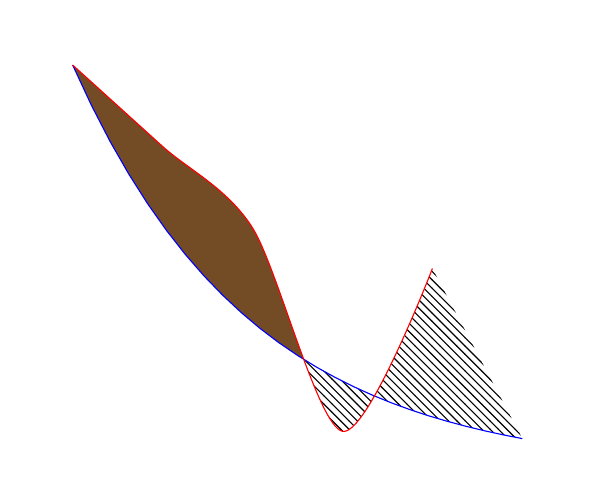
\begin{tikzpicture}
\begin{axis}[hide axis]
    \addplot[blue,name path=A,domain=0:5] {10*exp(-0.5*x)};
    \addplot[red,name path=B,smooth] table {
        x y
        0 10
        1 8
        2 6
        3 1
        4 5
    };
    \addplot fill between[of=A and B,
    split,
    %every odd segment /.style={yellow},];
    every segment no 3/.style={pattern color=gray!50,pattern=north east lines},
    every segment no 1/.style={pattern=north west lines},
    every segment no 2/.style={pattern=north west lines}
    ];
\end{axis}
\end{tikzpicture}
\end{document}